% Define document class
\documentclass[usenatbib,fleqn,letters]{mnras}
\usepackage{showyourwork}
\usepackage{graphicx}
\usepackage{amssymb,amsmath}
\usepackage{color}
\usepackage{multirow}
\usepackage{soul}
\usepackage{orcidlink}
\usepackage{comment}


\newcommand{\sarc}{$^{\prime\prime}\!\!$}
\newcommand{\myreferences}{references.bib}
\newcommand{\frii}{FR$\,$II}
\newcommand{\fri}{FR$\,$I}
\newcommand{\wphz}{$\,$W$\,$Hz$^{-1}$}
\newcommand{\tbpeak}{$T_{b,\mathrm{peak}}$}
\newcommand{\tbtotal}{$T_{b,\mathrm{total}}$}
\newcommand{\muJybm}{$\mu$Jy$\,$beam$^{-1}$}

\defcitealias{morabito_identifying_2022}{M22}
\defcitealias{best_lofar_2023}{B23}

% Title
\title[TBD]{TBD}

% Author list
\author[L.K. Morabito]{\parbox{\textwidth}{Leah K. Morabito$^{1,2}$\thanks{E-mail: leah.k.morabito@durham.ac.uk}\orcidlink{0000-0003-0487-6651}\\}\\ 
$^{1}$Centre for Extragalactic Astronomy, Department of Physics, Durham University, Durham DH1 3LE, UK \\
$^{2}$Institute for Computational Cosmology, Department of Physics, Durham University, South Road, Durham DH1 3LE, UK \\ }

% Begin!
\begin{document}

\date{}
\pagerange{\pageref{firstpage}--\pageref{lastpage}} \pubyear{2021}
\maketitle

\label{firstpage}


% Abstract with filler text
\begin{abstract}
    TBD
    \vspace{6.75in}
\end{abstract}




% Main body with filler text
\section{Introduction}
\label{sec:intro}
The extent to which active galactic nuclei (AGN) impact galaxy formation is a major open question in astrophysics. It is clear that there is an interaction, from both observational and theoretical standpoints. Observations have revealed tight scaling relations between the mass of a super-massive black hole and its host galaxy \citep[see, e.g.][and references therein]{kormendy_coevolution_2013}, while cosmological simulations require some form of AGN feedback \citep{bower_breaking_2006,croton_many_2006} to be able to reproduce the observed galaxy population. Galaxies build up their stellar mass through star formation, while super-massive black holes are expected to provide either negative or positive feedback \hl{citations!} to either suppress or stimulate galaxy growth. 

However, if one wishes to study the cosmic history of AGN activity or star formation (SF), and by extension the interplay between them, it is necessary to measure each process separately. This is a difficult problem at any wavelength. For example \hl{mid-infrared}. Multi-wavelength approaches use spectral energy distribution (SED) fitting, which utilises information from a broad number of observed bands to jointly fit galaxy and AGN components \citep{pacifici_art_2022}. \hl{give a couple of examples} \citep{calistro_rivera_agnfitter_2016,boquien_cigale_2019}. However, SED fitting is costly as it relies on observations using many different instruments over the same part of the sky, which then have to be carefully cross-matched. Selection effects at different bands can also present a problem. 


%% suggestion from Ryan: MIR community - AGN fraction


An alternative method to unambiguously identify the AGN component(s) in a galaxy is through brightness temperature, $T_b$, measurements in the radio waveband. Radio emission has the advantage of being unobscured by dust or gas, meaning there are minimal selection effects. Brightness temperature is a non-physical temperature which is defined as the temperature of a blackbody which would produce the observed surface brightness. Models of radio emission from SF predict an upper limit to the surface brightness that can be produced, even in starburst galaxies \citep{condon_radio_1992}. Surface brightness which is detected above this limit therefore has to be attributed to AGN activity. Brightness temperature is inversely proportional to frequency and resolution, $T_b \propto \nu^{-2}\Omega^{-1}$ (where $\Omega \propto \theta_{maj}\theta_{min}$). Traditionally brightness temperature measurements require Very Long Baseline Interferometry (VLBI) which achieve milli-arcsec resolutions at GHz frequencies \hl{citations} to achieve enough sensitivity to make meaningful measurements. In \cite[][hereafter, \hl{M22}]{morabito_identifying_2022} we demonstrated using sub-arcsecond resolution (0.\sarc\ 3) at 144 MHz with the LOw Frequency ARray \citep[LOFAR;][]{van_haarlem_lofar:_2013}. The advantage of LOFAR is its wide field of view: $\sim$6 deg$^2$ from a single observation versus a few to a couple hundred arcmin$^2$ with VLBI at GHz frequencies, depending on whether one is imaging at the phase centre of the observation or using multi-phase centres for correlation \hl{citations}. For example, using an 8 hour LOFAR observation of the Lockman Hole \citep{sweijen_deep_2022} we identified 940 AGN via brightness temperature \citepalias{morabito_identifying_2022}, providing a sample two orders of magnitude larger than any VLBI sample of AGN identified at GHz frequencies. 

As part of the LOFAR Two-metre Sky Survey Deep Fields \citep{sabater_lofar_2021,tasse_lofar_2021} campaign, we have now doubled the areal coverage of 0.\sarc\ 3 resolution wide-field imaging. \cite{de_jong_into_2024} recently published their 0.\sarc\ 3 resolution image of the ELAIS-N1 field, which reaches a depth of 14 $\mu$Jy$\,$bm$^{-1}$ using 32 hours of observations. They also demonstrate the flexible resolution which can be achieved with LOFAR, by imaging at 0.\sarc\ 6 and 1.\sarc\ 2 resolution, which are both complementary to the existing 6\sarc\ \ Deep Fields Data Release 1 (DR1). Again this has an advantage over VLBI with instruments at GHz frequencies, which require either observing at lower frequency bands (e.g., e-MERLIN) or with other instruments (e.g., EVN, VLBA) to acquire information on the flux density of sources at other scales. As described in \S~5 of \citepalias{morabito_identifying_2022}, for sources which are unresolved in the 0.\sarc\ 3 resolution images and do not exhibit a radio excess over that predicted the star formation rate (SFR) derived from SED fitting \citep[see][for more details]{best_lofar_2023}, we can separate the AGN activity from SF using a combination of the 0.\sarc\ 3 and 6\sarc\ \ resolution images. 


The 2,483 sources in Lockman Hole \citep{sweijen_deep_2022} and now the 13,058 sources in ELAIS-N1 \citep{de_jong_into_2024}, represents a massive step towards robust statistical studies where the population can be broken into bins of redshift and stellar mass to investigate AGN activity and SF.\cite{cochrane_lofar_2023} and \cite{kondapally_cosmic_2022} constructed radio luminosity functions (RLFs) from the 6\sarc\ \ resolution imaging that formed the Deep Fields DR1 for the star forming galaxies and radio-excess AGN, respectively.  Here we are able to reproduce those RLFs and further construct RLFS by activity -- either AGN or SF -- rather than by overall galaxy classification. This is the first time such RLFs have been constructed from observations, and provides insight into the non-radio excess population. These RLFs by activity also afford us the opportunity for a more direct comparison with cosmological simulations like SIMBA \hl{Nicole, citations} or EAGLE \hl{citations}. We can also investigate the cosmic evolution of AGN activity and SF by dividing the sample into redshift bins. 

In this paper, we first describe the data and methods in \S~\ref{sec:data}. We use a ... 

Throughout this paper, we use a $H_0 = 70$ km$\,$s$^{-1}\,$Mpc$^{-1}$, $\Omega_M = 0.3$, and $\Omega_{\Lambda}= 0.7$ cosmology. 

%Stuff and things \citep{morabito_sub-arcsecond_2022}.

\section{Data}
\label{sec:data}

\subsection{LoTSS Deep Fields DR1}
\label{subsec:dr1}
The LOFAR Two-metre Sky Survey (LoTSS) has both a wide-area \citep{shimwell_lofar_2017,shimwell_lofar_2021,shimwell_lofar_2022} and Deep Fields \citep{tasse_lofar_2021,sabater_lofar_2021} component. The Deep Fields Data Release 1 (DR1) in 2021 included Boötes, Lockman Hole, and ELAI-N1, reaching sensitivities of 30, 23, and 20 \muJybm , using $\sim$80, $\sim$100, and $\sim$160 hours, respectively. Alongside these deep radio images and their associated catalogues, \cite{kondapally_lofar_2021} provided a careful compilation of the ancillary deep data at other wavebands (from far-infrared to ultraviolet) and cross-matching to the radio catalogues, followed by photometric redshifts and stellar mass estimates in \cite{duncan_lofar_2021}. Collectively these catalogues provide an excellent resource, and we refer the reader for more details to the individual papers cited above.

Based on the cross-matched multi-wavelength catalogue \citep{kondapally_lofar_2021}, \cite[][hereafter, B23]{best_lofar_2023} carried out detailed SED fitting for all radio-detected sources across the three deep fields, using the multi-wavelength data. Full details can be found in their paper, but here we outline the relevant details. All sources detected above 5$\sigma$ in their respective radio images had their far-infrared (FIR) to ultraviolet (UV) data fit using four different SED fitting software packages. These were: MAGPHYS \citep{da_cunha_simple_2008}, BAGPIPES \citep{carnall_inferring_2018,carnall_how_2019}, CIGALE \citep{burgarella_star_2005,noll_analysis_2009,boquien_cigale_2019}, and AGN\textsc{fitter} \citep{calistro_rivera_agnfitter_2016}. The first two (MAGPHYS and BAGPIPES) use an energy balance approach, where optical to UV energy absorbed by dust must be transferred to thermal emission in the FIR to sub-mm.  CIGALE also uses the same energy-balance approach, but includes an AGN component. The final code, AGN\textsc{fitter} is designed to work in cases where the UV light and IR emission are spatially distinct, and thus the energy balance assumption does not hold. Many AGN fall under this umbrella. Each galaxy was fit with all four codes (twice for CIGALE, using different AGN components) and a `consensus' value found for the derived galaxy properties using information from the goodness-of-fits.  

The derived consensus properties used in this paper are \hl{stellar masses} and SFRs. We also use the galaxy classifications which arise from the SED fitting. \citetalias{best_lofar_2023} use the relationship between radio luminosity and SFR to define sources as either \textit{radio excess} or not. The AGN components used to fit the multi-wavelength information indicate whether a source is a radiatively efficient AGN (i.e., is there evidence for a disk/torus structure) or not. Combining these provides the following classes:
\begin{itemize}
    \item Radio excess + radiatively efficient
    \item Radio excess + not radiatively efficient
    \item Radiatively efficient + not radio excess
    \item Radiatively inefficient + not radio excess
\end{itemize}
The first three classes are AGN, and the final class is star forming galaxies (SFGs). The third class, radiatively efficient + not radio excess, are what are commonly called `radio-quiet' (RQ) AGN, while the first two AGN classes would be considered `radio-loud' (RL).  We note here that this is an observational classification scheme where RL-AGN have radio emission which is not consistent with SF, but that does not mean that the RQ-AGN do not have an AGN component -- which we will return to in \S~\hl{tbd}. 


\subsection{0.\sarc\ 3 resolution imaging}
\label{subsec:highres}

Data for LoTSS is recorded with all available LOFAR stations, which are spread across nine different European countries, with a preponderance of \textit{core} and \textit{remote} stations at the heart of the array in the Netherlands. The longest baseline (currently Ireland to Latvia) is $\sim$2,000 km, providing unprecedented resolution at MHz frequencies. While LoTSS uses only the stations in the Netherlands for its standard data processing, it is becoming stahdard to use the full array to achieve sub-arcsecond resolution \citep[e.g.,][]{morabito_sub-arcsecond_2022} on individual targets. We are currently post-processing LoTSS data to include the full international array where available. 

Post-processing of LoTSS data to achieve sub-arcsecond resolution ongoing for all Deep Fields, where we image the full field of view available to the international array. Due to the fact that the station layout of international stations is larger than that of stations in the Netherlands, the station beams naturally have a smaller field of view. Coupled with bandwidth and time smearing, this limits the field of view effectively to a radius of 1.24 deg, which still provides $\sim$5-6 deg$^2$ of coverage. 

The Lockman Hole was the first field to have its full field of view imaged at 0.\sarc\ 3 resolution \citep{sweijen_deep_2022}. This took a quarter million cpu hours to produce a single 7-billion pixel image from 8 hours of data. The resulting image has a median rms noise of 34 \muJybm , although this is lower in the centre and higher in the outskirts. It is useful to note that this image is deeper than an image at 6\sarc\ \ resolution using the exact same 8 hours of data, as adding the international stations increases the collecting area and therefore the sensitivity of the array. From this image, a catalogue of 2,316 5$\sigma$ sources was created, removing duplicates and grouping individual Gaussian islands together into sources. 

The first 0.\sarc\ 3 image of ELAIS-N1 has recently been published \citep{de_jong_into_2024}, along with companion images at intermediate resolutions of 0.\sarc\ 6 and 1.2\sarc . The median rms noise reaches 14 \muJybm\ in the centre of the 0.\sarc\ 3 resolution image, and increases radially. For consistency with the Lockman Hole sample, we do not use the intermediate resolution images here. In the 0.\sarc\ 3 resolution image, there were 13,058 sources catalogued above 5$\sigma$ after grouping Gaussian islands into sources and removing duplicates. 

Thanks to the added collecting area of the international stations, the 0.\sarc\ 3 resolution image made with 32 hours of data is now \textit{deeper} than the 6\sarc\ \ resolution image made with $\sim$160 hours of data. The derived galaxy properties from \citetalias{best_lofar_2023} (see \S~\ref{subsec:dr1}) were for LoTSS Deep Fields DR1, and thus we have to limit the source catalogue we wish to use. 

For both Lockman Hole and ELAIS-N1 catalogues derived from the 0.\sarc\ 3 resolution images, we first find the local rms in the 6\sarc\ \ resolution noise map\footnote{\label{dr1}Available at \href{https://lofar-surveys.org/deepfields.html}{https://lofar-surveys.org/deepfields.html}} at the position of each source. Using the peak brightness of the source in the catalogue from the 0.\sarc\ 3 resolution image, we calculate the peak-to-noise ratio and only select sources which would be detectable at the 5$\sigma$ limit. This ensures we do not have sources in the 0.\sarc\ 3 resolution catalogue which do not have a match in DR1. We then cross-match based on radio position, to provide the radio information from the catalogues derived from both the 0.\sarc\ 3 resolution image and the 6\sarc\ \ resolution image. We trim the area down for each field using their respective optical starmasks\textsuperscript{\ref{dr1}}, by selecting sources which are not contained in the null areas of these masks. This removes sources where the multi-wavelength information is impacted by bright stars. Finally, we trim the area down to the 2.5 deg$\times$2.5 deg area which is covered by the 0.\sarc\ 3 resolution image. 

Finally, we determine whether sources are resolved or unresolved in the same manner as \S~3.1 of \cite{shimwell_lofar_2019,shimwell_lofar_2022}. Truly unresolved sources in radio maps should have a peak brightness to integrated flux density ratio of unity, but LOFAR maps are impacted by smearing due to the ionosphere. This causes resolved sources to have a lower peak brightness to integrated flux density ratio, and they can appear slightly extended in the radio images. We start by selecting sources which are fit by single Guassian ({\ttfamily S\_CODE = 'S'}), and make a cut to remove sources which are larger than a multiple of the beam size. For the Lockman Hole, we use a factor of 3, but for ELAIS-N1 we find that a factor of 4 provided a better sample. This may be because half of the data for ELAIS-N1 had been pre-averaged to 2 sec integration times, which will increase the time smearing \citep[see \S~2 in][]{de_jong_into_2024}. We fit a sigmoid function to find the upper 99.9th percentile of sources considering their integrated flux density to peak brightness ratio as a function of the local signal to noise. \hl{The fit parameters and graphical representation of the data can be found in the supplemental online materials.}

We are left with \hl{fill in} sources in Lockman Hole, and \hl{fill in} sources in ELAIS-N1. We use the source name from the catalogue derived from the 6\sarc\ \ resolution to cross-match to the catalogue from \citetalias{best_lofar_2023}. 

\subsection{Simulations}
\hl{Nicole}

\section{Methods}

Brightness temperature, $T_b$, is used to characterise the surface brightness of radio emission. It is not a physical temperature, but rather the temperature of a black body  which would produce the observed spectral radiance (assuming the Rayleigh-Jeans approximation) at long wavelengths. By creating a model which predicts the upper limit of $T_b$ achievable by star formation \citep[based on][]{condon_radio_1992}, if the value is \textit{above} that upper limit, the radio emission must be due to AGN activity.  \citetalias{morabito_identifying_2022} showed that this AGN identification can be done at 150 MHz using sub-arcsecond resolution; this works because $T_b\propto\nu^{-2}\Omega^{-1}$ where $\nu$ is the observed frequency and $\Omega$ is the solid angle of the emitting region -- for unresolved sources, this corresponds to the deconvolved beam size. We refer the reader to \S~3 of \citetalias{morabito_identifying_2022} for more details, but note that this method yields conservative, positive AGN identifications. There may be lower surface brightness AGN emission which is not identified, and it is also possible \citep[although unlikely, according to][]{condon_radio_1992} that extreme, compact nuclear starbursts could produce AGN-like values of $T_b$. 

\subsection{Separation of AGN activity and SF}
Once the AGN activity is identified from the 0.\sarc\ 3 resolution images, it is possible to separate it from star formation using the total flux density from the 6\sarc\ \ resolution images. We refer the reader to \S~5 in \citetalias{morabito_identifying_2022} for more details but outline the process here. Sources which are identified as radio excess according to the definition in \citetalias{best_lofar_2023} automatically have their total flux density from the 6\sarc\ resolution images added to the AGN category. For sources that are not radio excess, we attribute the total flux density from the 6\sarc\ resolution images to SF if in the 0.\sarc\ \ 3 resolution image they are: resolved, multi-component, or have no detection. Sources which do not meet these criteria (i.e., unresolved single component) are checked and if their $T_b$ is not above the limit for SF their 6\sarc\ resolution total flux density is also added to the SF category. The total flux density of any source in the 0.\sarc\ 3 resolution image which is $T_b$-identified AGN is assumed to be AGN flux density; this is subtracted from the total flux density measured from the 6\sarc\ \ resolution image, and what remains is assumed to be flux density from SF. Fig.~\ref{fig:flowchart} shows a flowchart of how flux density is assigned to either the AGN or SF category. 

\begin{figure}
    \centering
    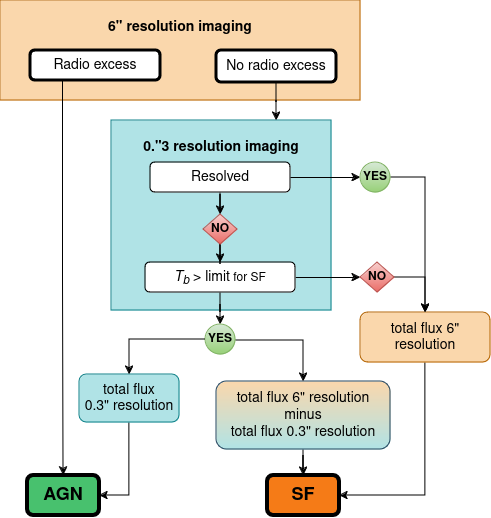
\includegraphics[width=0.5\textwidth]{figures/agn_sf_separation_workflow.png}
    \caption{Caption}
    \label{fig:flowchart}
\end{figure}

\subsection{Construction of RLFs}

We follow the same method of constructing RLFs as in \cite{kondapally_cosmic_2022} and \cite{cochrane_lofar_2023}. As the 0.\sarc\ \ 3 resolution image is smaller than the 6\sarc\ resolution image, we first reproduce the published RLFs (Fig.~\ref{fig:rlfs}, left panel) using the galaxy classifications from \citetalias{best_lofar_2023} to check that we have implemented the method appropriately, and that the smaller area yields the same results. We use the completeness corrections from the respective papers. The only correction we do not implement is the photo-$z$ correction used in \cite{cochrane_lofar_2023}. The authors note that this correction is negligible, and as it is not implemented in \cite{kondapally_cosmic_2022} we chose to keep the method for RLF construction in this paper consistent across both samples. We use the same redshift range, $0.003 < z < 0.3$ and see that we indeed have good agreement with the published RLFs.

Next we use the same method for constructing RLFs by activity rather than overall galaxy classifcation. We again use the completeness corrections from \cite{cochrane_lofar_2023} and \cite{kondapally_cosmic_2022}. The completeness corrections are flux density dependent, and we use the overall total flux density of a galaxy, rather than the flux density of the activity (which may be smaller if there are both AGN and SF components). This is because completeness corrections are based on whether or not a \textit{source} will be detectable given the background rms. This only relies on the total flux density, not the flux density of individual components. The RLFs by activity rather than galaxy classification are shown in the middle panel of Fig.~\ref{fig:rlfs}, again for  $0.003 < z < 0.3$. 

Finally, we use RLFs constructed from SIMBA. The RLFs are constructed as in \cite{thomson_radio_2019}, but have been updated to use the same redshift bins \hl{Nicole}. 

\section{Results}

To illustrate the differences in RLFs constructed by activity vs. by galaxy classification we divide the activity RLF by the galaxy RLF and show the ratio in the bottom right hand panel in Fig.~\ref{fig:rlfs}, for both the AGN and SF category. We see that above 10$^{24}\,$\wphz\ the ratio for AGN is unity, which is expected where radio excess sources dominate the population. Below that, the ratio for AGN climbs up to $\sim$1.25 and finally almost up to 2 at the lowest radio powers probed. The ratio for SF is always below unity, but it does not deviate as much as the ratio for AGN. This is because the SF population has larger source counts, so the total impact of moving some flux density from the SF to AGN population is less extreme. 

In Fig.~\ref{fig:agn_evolution} we show 



%- sfrd, kinetic LF

%\begin{figure}
%    \centering
%    \includegraphics[width=0.5\textwidth]{figures/simba_comparison.png}
%    \caption{Caption}
%    \label{fig:simba}
%    \script{simba_comparison.py}
%\end{figure}

\begin{figure*}
    \centering
    \includegraphics[width=0.98\textwidth]{figures/deep_fields_RLFs.png}
    \caption{Caption}
    \label{fig:rlfs}
    \script{comparison_plot.py}
\end{figure*}

\begin{figure*}
    \centering
    \includegraphics[width=0.49\textwidth]{figures/RLF_evolution_SF.png}
    \includegraphics[width=0.49\textwidth]{figures/RLF_evolution_AGN.png}
    \caption{Caption}
    \label{fig:sf_evolution}
    \script{RLF_evolution_v2.py}
\end{figure*}


\section{Discussion and conclusions}


\section*{Data Availability}
Reference showyourwork on github

\section*{Acknowledgements}
LKM is grateful for support from UKRI [MR/T042842/1]. 

LOFAR is the Low Frequency Array designed and constructed by ASTRON. It has observing, data processing, and data storage facilities in several countries, which are owned by various parties (each with their own funding sources), and which are collectively operated by the ILT foundation under a joint scientific policy. The ILT resources have benefited from the following recent major funding sources: CNRS-INSU, Observatoire de Paris and Université d'Orléans, France; BMBF, MIWF-NRW, MPG, Germany; Science Foundation Ireland (SFI), Department of Business, Enterprise and Innovation (DBEI), Ireland; NWO, The Netherlands; The Science and Technology Facilities Council, UK; Ministry of Science and Higher Education, Poland; The Istituto Nazionale di Astrofisica (INAF), Italy.

This research made use of the Dutch national e-infrastructure with support of the SURF Cooperative (e-infra 180169) and the LOFAR e-infra group. The Jülich LOFAR Long Term Archive and the German LOFAR network are both coordinated and operated by the Jülich Supercomputing Centre (JSC), and computing resources on the supercomputer JUWELS at JSC were provided by the Gauss Centre for Supercomputing e.V. (grant CHTB00) through the John von Neumann Institute for Computing (NIC).

This research made use of the University of Hertfordshire high-performance computing facility and the LOFAR-UK computing facility located at the University of Hertfordshire and supported by STFC [ST/P000096/1], and of the Italian LOFAR IT computing infrastructure supported and operated by INAF, and by the Physics Department of Turin university (under an agreement with Consorzio Interuniversitario per la Fisica Spaziale) at the C3S Supercomputing Centre, Italy.


\begin{comment}
\section*{Appendix A}

\begin{figure*}
    \includegraphics[width=0.49\textwidth]{figures/Lockman_Unresolved_03.png}
    \hfill
    \includegraphics[width=0.49\textwidth]{figures/ELAIS_Unresolved_03.png}
    \caption{\label{fig:unres}The data and sigmoid fits to determine whether sources are resolved or unresolved as described in \S~\ref{subsec:highres}. The \textit{left} panel shows Lockman Hole, and the \textit{right} panel shows ELAIS-N1. }
\end{figure*}

Figure~\ref{fig:unres} shows the integrated flux density to peak brightness ratio as a function of the local signal to noise, parameterised by $\frac{S_{peak}}{2\sigma_{peak}} + \frac{S_{int}}{2\sigma_{int}}$. The data is first binned evenly in log space, and the 99.9th percentile is found in each bin. We then fit a sigmoid function:
\begin{equation}
y = A + \frac{B}{1 + (x / 96.57)^C}, 
\end{equation}
where 96.57 is a fixed value that has worked well for LoTSS \citep{shimwell_lofar_2022}. For Lockman Hole, we find 
\end{comment}

\clearpage
\pagebreak


\bibliographystyle{mnras}
\bibliography{references}


\label{lastpage}

\end{document}
